\section{Class Diagrams}
The class diagrams are a visual representation on how the RRS has been structured. The project overview given below shows which modules are submodules from the overheading modules. In the UML diagrams below there has been given a precise and complete overview of the class diagrams per module. These diagrams have been made using a generating tool in a command line interface.

\subsection{Project Overview}

\includegraphics[width=\linewidth]{project-overview.png}

\subsection{Controller - Steam Controller}
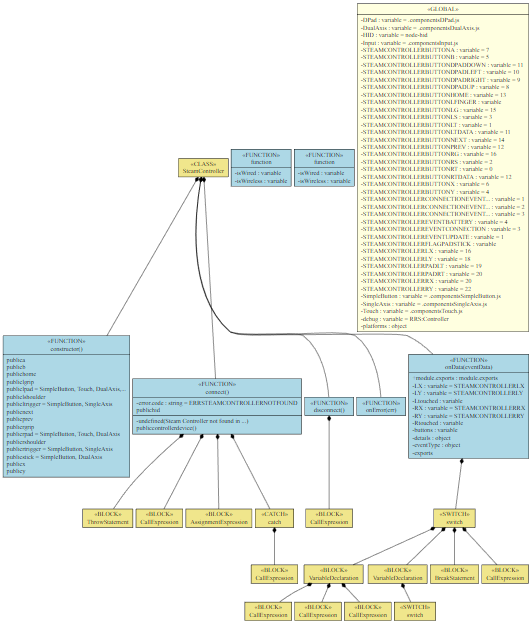
\includegraphics[width=\linewidth]{controller-steamcontroller.PNG}

\subsection{Controller - DPad}
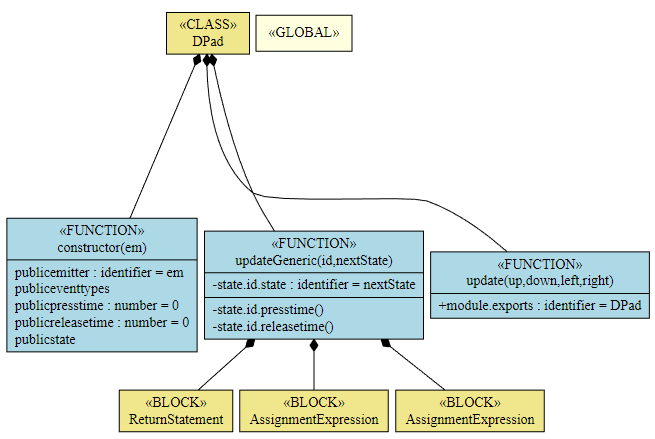
\includegraphics[width=\linewidth]{controller-dpad.PNG}

\subsection{Controller - Dual Axis}
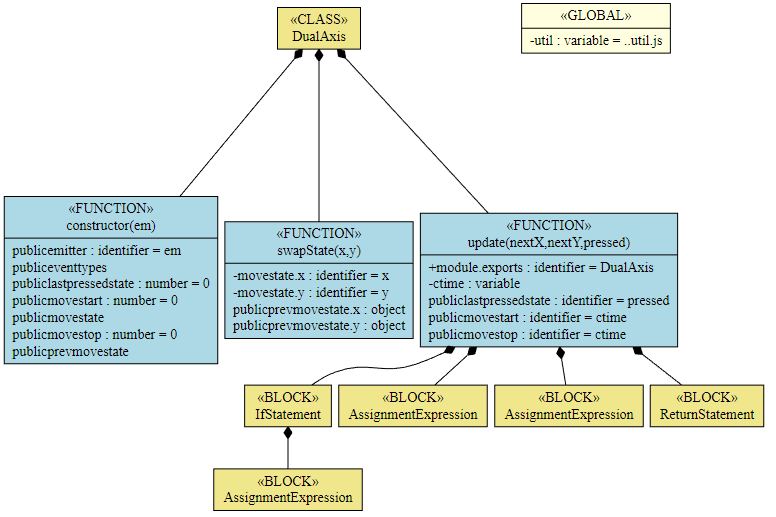
\includegraphics[width=\linewidth]{controller-dualaxis.PNG}

\subsection{Controller - Simple Button}
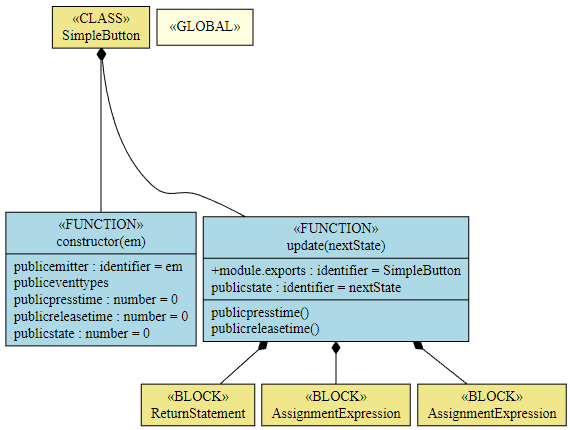
\includegraphics[width=\linewidth]{controller-button.PNG}

\subsection{Controller - Touch}
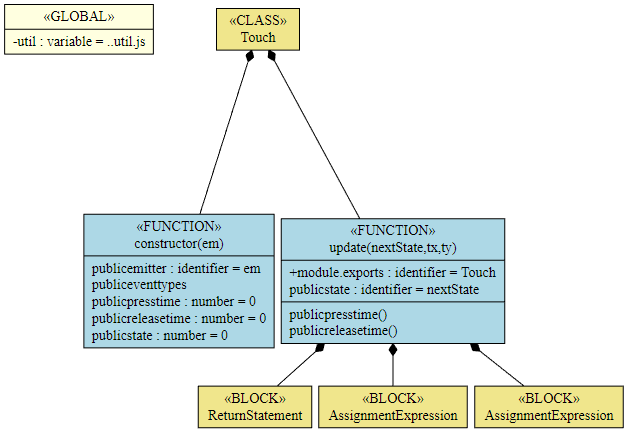
\includegraphics[width=\linewidth]{controller-touch.PNG}

\subsection{Controller - Single Axis}
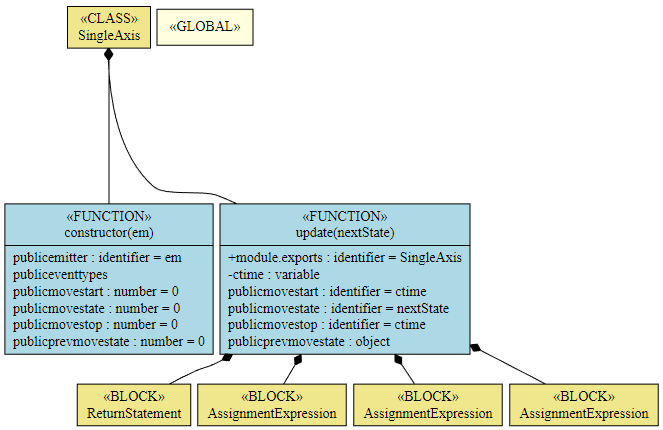
\includegraphics[width=\linewidth]{controller-singleaxis.PNG}

\newpage
\subsection{Motor}
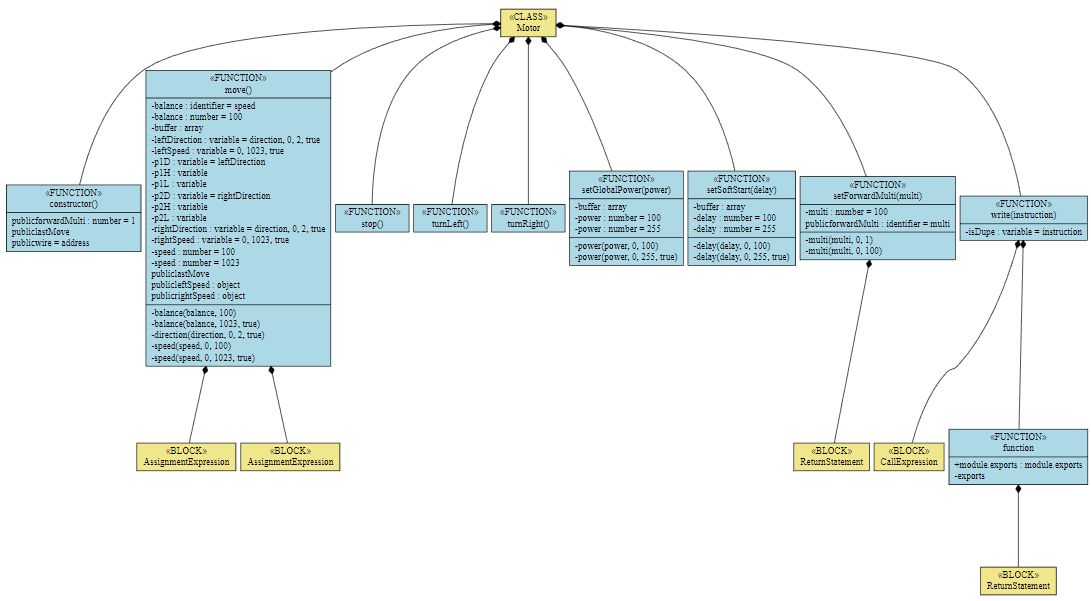
\includegraphics[width=\linewidth]{diagram-motor.PNG}

\newpage
\subsection{Nervi - Camera Mount}
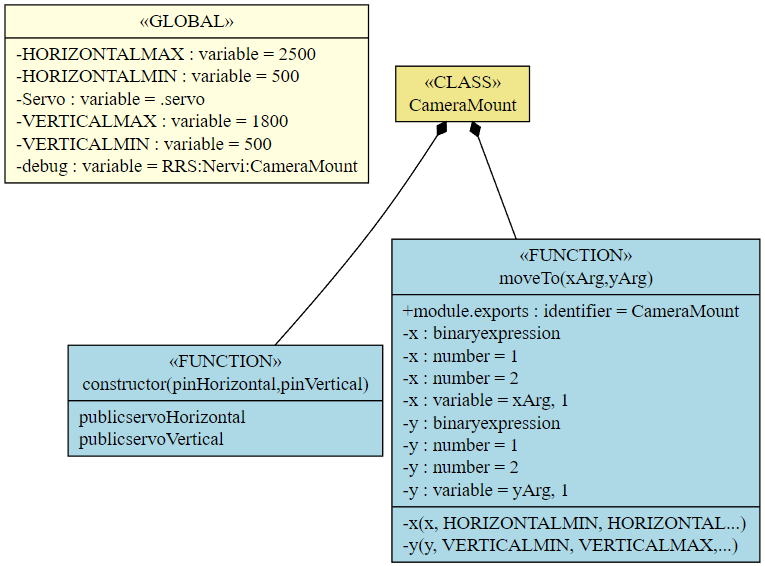
\includegraphics[width=\linewidth]{diagram-nervi-cameramount.PNG}

\subsection{Nervi - Rotary Encoder}
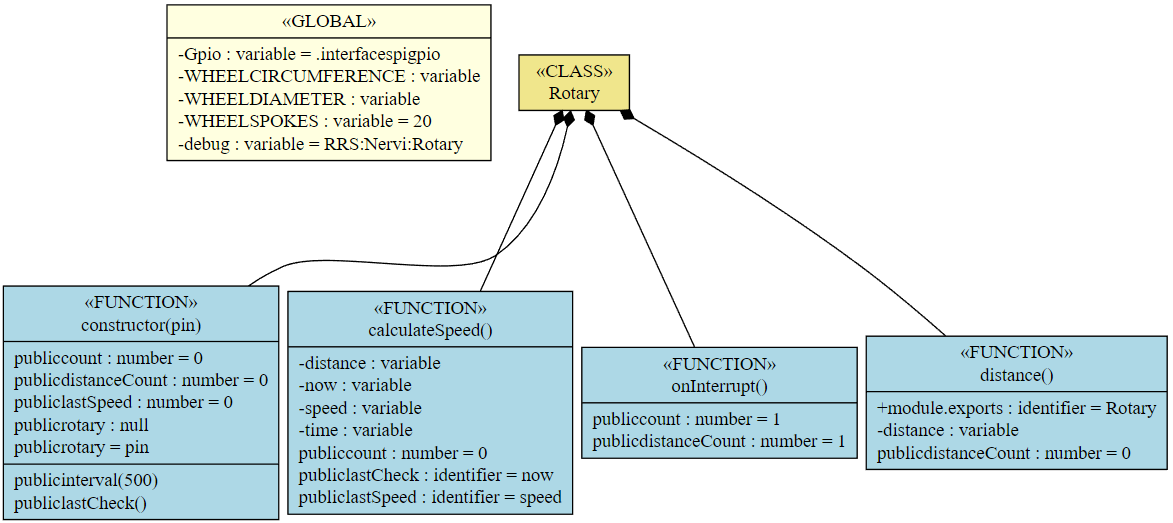
\includegraphics[width=\linewidth]{diagram-nervi-rotary.PNG}

\subsection{Nervi - Servo}
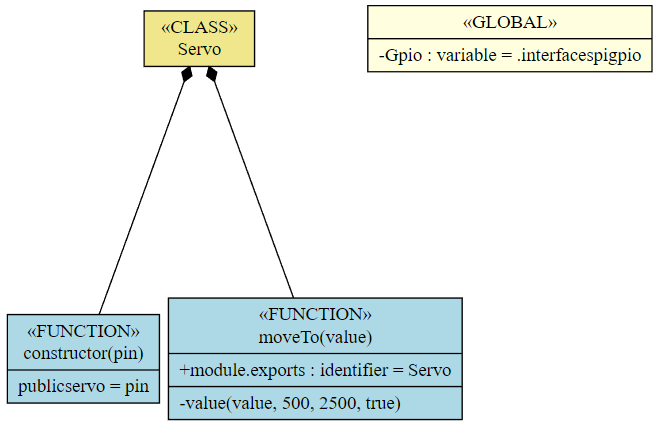
\includegraphics[width=\linewidth]{diagram-nervi-servo.PNG}

\subsection{Nervi - Ultrasonic}
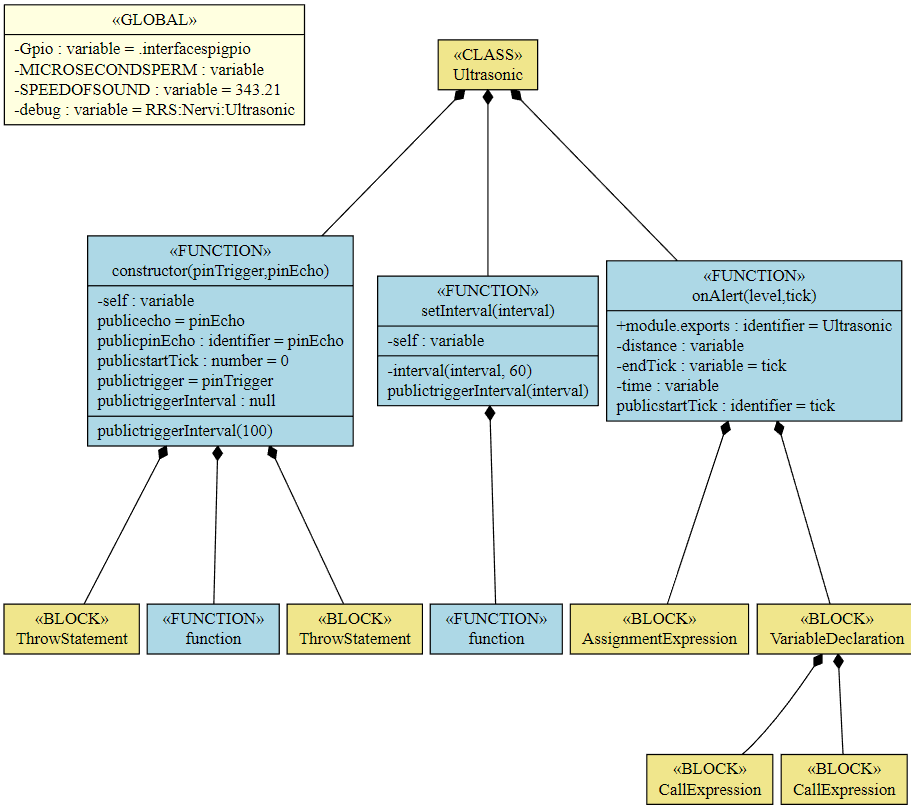
\includegraphics[width=\linewidth]{diagram-nervi-ultrasonic.PNG}
